% !TEX root = pfe-book2.tex
%!TEX TS-program = pdflatex
%!TEX encoding = UTF-8 Unicode


\cleardoublepage
%\mainmatter
\chapter{Building Blocks of the Universe}
\label{ch-01}

\section{Elements}
What is the world surrounding us made of? The first answers to this question which have reached us originat­ed in Ancient Greece more than 25 centuries ago.

At first glance, the answers seem as strange as can be, and we would have to waste a lot of paper in order to explain to the reader the logic of the ancient sages -- Thales, having asserted that everything consists of water, Anaximander, having said that the world is made of air, or Heraclitus, in whose opinion every­ thing consists of fire.

The incongruity of such explanations forced later Greek ``lovers of wisdom'' (that’s how the word ``philos­opher'' is translated) to increase the number of funda­mental principles or, as they were called in antiquity, elements. Empedocles asserted that there are four ele­ments: earth, water, air and Fire. Aristotle contributed the final (for a very long time) corrections to this in­vestigation.

According to Aristotle, all bodies consist of one and the same substance, but this substance can assume finalities. There are four immaterial elements: cold, hot moist and dry. Combining in pair and being imparted to a substance, Aristotle’s elements form the
elements of Empedocles. Thus, a dry and cold substance
yields earth, dry and hot fire; moist and cold, water and finally, moist and hot, air.

However, in view of the difficulty involved in an­swering many questions, ancient philosophers added a ``divine quintessence'' to the four elements. This was a kind of god-cook, cooking the various elements together. Of course, it isn’t hard to explain away any perplexity by reference to a god.

But for a very long time -- almost up to the 18th cen­tury -- few dared be perplexed and ask questions. Aris­totle’s teachings were avowed by the Church, and any doubt in their validity was a heresy.

But these doubts arose anyway. They were engendered by alchemy.

In the distant past, into the heart of which we can look by reading ancient manuscripts, people knew that all bodies surrounding us were capable of being trans­formed into others. Combustion, sintering, the melting of metals -- all these phenomena were well known.

This, it would seem, did not contradict Aristotle’s teaching. The so-called ``dosage'' of the elements changed during any transformation. If the whole world consists of only four elements, the possibilities of transforming bodies should be very great. It is merely necessary to find the secret of what to do in order that any body might be obtained from any other one.

How tempting is the problem of making gold or find­ing a special, extraordinary ``philosophers' stone'', giving its possessor wealth, power and eternal youth. The science of manufacturing gold and a philosophers' stone, of transforming any body into any other one was called alchemy by the ancient Arabs.

The labour of people devoting themselves to the so­lution of this problem continued for centuries. Alchemists did not learn how to make gold, did not find a philos­ophers' stone, but made up for this by collecting many valuable facts about the transformation of bodies. In the final analysis, these facts served as the death sentence for alchemy. In the 17th century, it became ob­vious to many people that the number of basic substances -- elements -- is incomparably greater than four. Mercury, lead, sulphur, gold and antimony turned out to be undecomposable substances; one could no longer say that these substances were made out of elements. On the contrary, one had to rank them among the ele­ments of the world.

In 1661 in England. Robert Boyle (1627-1691) pub­lished the book \emph{The Sceptical Chemist}. Here we find a completely new definition of an element. This is no longer the elusive, mysterious immaterial element of alchemists. An element is now a substance, a component part of a body. This is consistent with the modern def­inition of the concept of an element.

Boyle's list of elements was not very large. He added fire to a correct list. Incidentally, the idea of elements lived on even after Boyle. Even in a list of the great Frenchman Antoine Laurent Lavoisier (1743-1794), who is regarded as the founder of chemistry, side by side with real elements there also appear imponderable elements: heat-producing and light-producing substances.


In the first half of the 18th century, there were 15 known elements, and their number rose to 35 by the end of the century. True, only 23 of them were real elements but the rest were either non-existent elements or else substances like caustic soda and caustic potash which turned out to be compounds.

By the middle of the 19th century, more than 50 undecomposable substances were described in chemical handbooks.


The periodic law of the great Russian chemist Dmitri Mendeleev (1834-1907) provided the stimulus for a conscious search for undiscovered elements. It is still too early speak about this law here. Let us merely say that by means of his law Mendeleev showed how one must look for the elements which had not yet been dis­covered.

Almost all the elements occurring in nature were discovered by the beginning of the 20th century.


\section{Atoms and Molecules}

About 2000 years ago, an original poem was written in Ancient Rome. Its author was the Roman poet Lucre­tius. This poem was called \emph{On the Nature of Things}.

With sonorous lines Lucretius told of the ancient Greek philosopher Democritus’ views on the world in his poetic work.

What views were these? These were teachings about the minutest, invisible particles which our whole world is made of. Having observed various phenomena, De­mocritus tried to give them an explanation.

Take water for example. When sufficiently heated, it evaporates and disappears. How can this be explained? It is clear that such a property of water is related to its internal structure.

Or how, for example, can we perceive the scent of flowers at a distance? 

Meditating on similar questions, Democritus became convinced that bodies only seem to be solid, but in fact consist of the minutest particles.  These particles are different in form for different bodies, but they are
so small that they cannot be seen. That why all bodies seem to us to be solid.

Democritus called such very tiny particles which cannot be further divided and of which water and all other bodies consist \emph{atoms} (derived from the Greek \emph{atomos} meaning ``indivisible'').

This remarkable guess of ancient Greek thinkers, born 24 centuries ago was later long forgotten. Aristotle’s erroneous teaching exercised complete sway over the scientific world for more than a thousand years.

Asserting that all substances are mutually transmutable, Aristotle categorically denied the existence of atoms. Any body can be infinitely  divided, taught Aristotle.

In 1647 the Frenchman Pierre Gassendi (1592-1655)
published a book in which he courageously denied Aris­totle’s teaching and asserted that all substances in the world consist of small indivisible particles -- atoms. Atoms differ from each other in shape, size and mass.

Agreeing with the teachings of the ancient atomists, Gassendi developed these teachings further. He explained how the millions of diverse bodies of nature can and do arise in the world. For this, he asserted, a large number of different atoms is not necessary. For an atom is the same thing as building materials for houses. It is pos­sible to construct an enormous number of the most diverse houses from three different kinds of building mate­rial -- bricks, boards and logs. In precisely the same way nature can create thousands of the most diverse bodies from several tens of different atoms. Moreover, in each body various atoms are united in small groups; Gassendi called these groups \emph{molecules} i.e. ``small masses'' (derived from the Latin \emph{moles} meaning ``mass'').

Molecules of various bodies differ from each other in the number and kind (``sort'') of atoms belonging to them. It is not difficult to understand that an immense number of different combinations of atoms, molecules, can be created from several tens of different atoms. Which is 
why there is such a great variety of the bodies surrounding us.

However, Gassendi’s views still contained ideas that were incorrect. Thus, he believed that there are special atoms for heat, cold, taste and smell. As other scientists of that time he too could not completely free himself from Aristotle’s influence, and recognized his immaterial
elements.

The following ideas experimentally verified much later are contained in the writings of M. V. Lomonosov, the great enlightener and founder of science in Russia. 

Lomonosov writes that molecules can be homogeneous or heterogeneous. In the former case, similar atoms are grouped in a molecule. In the latter, a molecule consists of atoms differing from each other. If some body is composed of homogeneous molecules, it must be regarded as simple. If, on the contrary, a body con­sists of molecules built up from various atoms, Lomo­nosov calls it compound.

We now well know that nature’s various bodies have precisely such structure. In fact, take the gas oxygen for example; two identical atoms of oxygen are contained in each of its molecules. This is a molecule of a simple substance. But if the atoms composing a molecule are different, it is a chemical compound. Its molecules consist of atoms of those chemical elements which occur in the composition of this compound. This can also be said otherwise: each simple substance consists of atoms of one chemical element; a compound contains atoms of two or more elements.


A number of thinkers spoke about atoms, adducing logical arguments in favour of their existence. The English scientist John Dalton (1766-1844) introduced atoms into science in the right way and made them an object of research. Dalton showed that there exist chemical regularities which can be explained in a natural manner only by making use of the idea of an atom.

After Dalton, atoms firmly entered science. However, for a very long time there still were scientists who did not believe in atoms. Even at the very end of the last century, one of them wrote that after several decades it would be possible to find atoms only in the dust of libraries.

Such reasoning seems funny now. We know now so many details about the ``life'' of an atom that to doubt its existence is the same thing as to doubt the reality of the Black Sea.

The relative masses of atoms were determined by chemists. At first the mass of a hydrogen atom was taken as the atomic mass unit. The relative atomic mass of nitrogen turned out to be approximately equal to 14, oxygen, approximately 16, chlorine, approximately 35.5. A somewhat different choice of the relative atomic mass units was later made, for which the number 16.0000 was assigned to oxygen. The atomic mass of hydrogen turned out equal to 1.008 in this scale.

Of interest, of course, is the absolute mass of atoms and not only their relative mass. It is sufficient, for this purpose, to measure the absolute mass of an atom of any one kind. Taken as the basis today is carbon rather than oxygen or hydrogen. Up to the present time, investigators regarded measurements of absolute masses of atoms with distrust and proceeded as follows. They took the mass of the carbon isotope \ce{^{12}C} to be equal to exactly twelve atomic mass units (\si{\amus}). Then, paying no attention to the accuracy of measurement of the absolute masses of atoms, they assumed that
\begin{equation*}%
\SI{1}{\amus} = \SI{1.662e-24}{\gram}
\end{equation*}
In any case, this value does not differ appreciably from the true one. Perhaps they are overcautious, however, since the precision of measurement today is within a fraction of about one-millionth. Measuring techniques have advanced greatly during the last century. In 1875, the known value of \SI{1}{\amus} was accurate within about 30 percent.

How do we measure the mass of the atom in grams? No scales have been constructed, of course, on which a physicist could place a single atom and then balance it with a tiny weight. Like a hundred, years ago, physi­cists use indirect experiments for this purpose today as well. They are not, however, in any way less reliable than direct weighing would be. But we cannot do without any weighing at all. We put a solid ball of carbon \ce{^{12}C} on the scale rather than a single atom (actually we proceed in a somewhat different way, but the point is to explain the idea of weighing and so we hope the informed reader forgives our simplified description). When the mass of the ball and its size are known, we can determine its density. The substance being weighed must be a perfect crystal. This is not easy to achieve, but more or less feasible. Hence, we can evidently write the fol­lowing for the density found in the experiment
\begin{equation*}%
\rho = \frac{Z m_{A} }{V}
\end{equation*}
where $m_{A}$ is the mass of the atom in \si{\amus}, $V$ is the volume of a unit cell of the crystal, and $Z$ is the number of atoms per unit cell (see p. \pageref{unit-cell-def}). 

The last two quantities can be determined by $X$-ray structure analysis, which to be discussed in the fourth book.

The reader should not resent the fact that I seem to be getting ahead of my story. Books on physics should be read at least twice.

Employing this method, we can determine the atomic mass unit with exceptionally great precision. The most reliable value today is\footnote{The present (2022) estimate of amu is $(\num{1.66053906660} \pm \num{50})\times \SI{e-24}{\gram}$. -- Damitr}:
\begin{equation*}%
\SI{1}{\amus} = (\num{1.60043} \pm \num{0.00031})\times \SI{e-24}{\gram}
\end{equation*}
We now ask the reader to use his imagination in order to grasp the minuteness of this value. Assume that you demand a thousand million molecules from each person on earth. How much matter can you collect in this way? Only several thousandths of a millionth of a gram.

Or another such comparison: the earth is as many times heavier than an apple an apple is heavier than hydrogen atom.

The reciprocal of the atomic mass unit is called \emph{Avogadro's number}\footnote{The present (2022) estimate the Avogadro's number of is $\SI{6.02214076e23}{\per\mole}$. -- Damitr}:
\begin{equation*}%
N_{A} = \frac{1}{\si{\amus}} = \num{6.0220943e23}
\end{equation*}
This enormous number has the following significance. Let us take a substance of an amount in grams equal to the relative mass $M$ of its atoms or molecules, for example, 12 grams of the carbon isotope \ce{^{12}C}. This can be expressed more concisely: let us take one mole of a substance (check, please, with the definition of the mole given in the first book, where we introduced the International System of Units -- SI units). The mass of one mole of a substance is equal to $Mm_{A}$. Consequently the number of carbon atoms in 12 grams of carbon, as well as the number of atoms, molecules or any other particles in mole assembly of these particles, equals
\begin{equation*}%
\frac{M}{Mm_{A}} = N_{A}
\end{equation*}
which is Avogadro’s number.

For a long time physicists found no necessity for using
the concept of the ``amount of substance''. As long as we dealt only with atoms and molecules it was quite suitable to define the mole as the molecular (or atomic) weight expressed in grams.

But then ions, electrons, mesons and many, many more particles made their appearance. Physicists came to the conclusion that it is not always convenient to characterize an assembly of particles by their mass. This led to the establishment of the unit for the amount of substance -- the mole. When we speak of a mole of electrons, a mole of lead atom nuclei or a mole of pi-mesons, we are not specifying the mass of these particles (which, as you will find further on, depends upon their velocity), but only their number. The previous definition of a mole is still valid, however, because $N_{A}$ atoms or molecules of any kind have a mass equal practically to the atomic or molecular mass expressed in grams. Neither has Avogadro’s number changed its meaning; it simply has a new name: $\textrm{mole}^{-1}$.


\section{What Heat Is}

How does a hot body differ from a cold one? Up until the $19^{\textrm{th}}$ century, this question was answered as follows: ``A hot body contains more heat-producing matter (or `caloric') than a cold one, in exactly the same sense as soup is saltier if it contains more salt.'' But what is caloric? The following answer was given to this question: ``Caloric is the matter of heat, it is the elementary fire.'' Mysterious and incomprehensible. And this answer is in essence the same as the following explanation of what a rope is: ``A rope is simple `ropeness'.''

Along with the caloric theory, a different view on the nature of heat had long been in existence. It was brilliantly advocated by many outstanding scientists of the 16-$18^{\textrm{th}}$ centuries.

Francis Bacon wrote in his book \emph{Novum Organum}: ``Heat itself in its essence is nothing but motion\ldots{} Heat consists of a variable motion of the minutest particles of a body.''

Robert Hooke asserted in his book \emph{Micrographia}: ``Heat is a continuous motion of the parts of a body\ldots{} There is no such body whose particles would be at rest.''

We find particularly clear statements of this kind in Lomonosov’s work (1745) \emph{Reflections on the Cause of Heat and Cold}. The existence of caloric is denied in this work, where it is said that ``heat consists of the internal motion of particles of matter''.

Count von Rumford put it very graphically at the end of the 18th century: ``The more intensively the particles composing a body move, the hotter the body will be, analogous to how the more vigorously a bell vibrates, the louder it rings.''

In these remarkable guesses, far ahead of their time, the bases of our modern views on the nature of heat are concealed.

There are sometimes quiet and clear days. The leaves lie still on the trees, not even a slight ripple disturbs the glassy surface of water. The entire surroundings have frozen in strict, triumphant immobility. The visible world is at rest. But what is taking place in the world of atoms and molecules?

Contemporary physicists can say much about this. Never, not under any circumstances, is there a cessation to the invisible motion of the particles that the world is made of.

But why don’t we see all these motions? Particles move, but the body is stationary. How is this possible? 

Have you ever watched a swarm of midges? When there is no wind, the swarm appears to be suspended in air. But an intensive life is going on inside the swarm. Hundreds of insects flew off to the right, but just as many flew off to the left at the same instant. The swarm as a whole remained at the same place and did not change its form.

The invisible motions of atoms and molecules are of the same chaotic, irregular nature. If some molecules leave a volume, their place is occupied by others. But since the newcomers do not in the least differ from the departed molecules, the body remains entirely as it was. An irregular, chaotic motion of particles does not change the properties of the visible world.

``However, isn’t this idle talk?'' the reader might ask us. In what sense are these arguments, however beautiful, more convincing than the caloric theory? Has anyone actually seen the eternal thermal motion of particles of matter?

It is possible to see the thermal motion of particles and, moreover, with the aid of the simplest microscope. This phenomenon was first observed more than a hundred years ago by the English botanist Robert Brown (1773-1858).

Looking at the internal structure of a plant through a microscope, he noticed that tiny particles of matter floating in the sap of the plant were continually moving in all directions. The botanist became interested: what forces made the particles move? Perhaps they were living beings of some kind? The scientist decided to examine under a microscope small particles of clay making some water turbid. But neither were these un­doubtedly lifeless particles at rest; they were engaged in a continual and chaotic motion. The smaller the particles were, the faster they moved. The botanist examined this drop of water for a long time, but still he couldn’t see any end to the motion of the particles. Some invisible forces seemed to be constantly pushing them.

The Brownian movement of particles is just a thermal motion. Thermal motion is inherent in large and small particles, clots of molecules, individual molecules and atoms.


\section{Energy Is Conserved Forever}

Thus, the world is composed of moving atoms. Atoms possess mass, moving atoms possess kinetic energy. Of course, the mass of an atom is unimaginably small, and so its energy will also be minute, but there are millions of millions of millions of atoms.

We now remind the reader that although we spoke of the law of conservation of energy, this was not a sufficiently universal conservation law. Linear and angular momenta were conserved experimentally, but energy was only conserved ideally -- in the absence of friction. But as a matter of fact, energy always decreased.

But we did not say anything previously about the energy of atoms. A natural idea arises: where at first sight we noticed a decrease in energy, some energy was transmitted to the atoms of a body in a manner which is imperceptible to the naked eye.

Atoms are subject to the laws of mechanics. True (you will have to learn this from another book), their mechanics is somewhat peculiar, but this does not change matters -- with respect to the law of conservation of mechanical energy, atoms do not differ at all from large bodies.

Hence, the complete conservation of energy will be detected only when along with the mechanical energy of a body the internal energy of this body and the en­vironment is taken into account. Only in this case will the law be universal.

What does the total energy of a body consist of? We have, in essence, already named its first component -- it is the sum of the kinetic energies of all its atoms. But it must not be forgotten that atoms interact with each other. Therefore, the potential energy of this interaction is added. Thus, the total energy of a body is equal to the sum of the kinetic energies of its particles and the potential energy of their interaction.

It is not difficult to comprehend that the mechanical energy of a body as a whole is only part of its total ener­gy. For when a body is stationary, its molecules do not stop moving and do not cease interacting with each other. The energy of the thermal motion of particles which remains in a stationary body and the energy of the interaction between the particles constitute the internal energy of the body. The total energy of a body is therefore equal to the sum of its mechanical and in­ternal energies.

The gravitational energy of a body is component part of its mechanical energy i.e. the potential energy of the interaction between its particles and the Earth.

Considering internal energy, we no longer detect vanishing of energy. When we consider nature through glasses magnifying the world millions of times, the picture seems to us to be of rare harmoniousness. There are no losses of mechanical energy, but there is only its transformation into the internal energy of a body or its surroundings. Has any work disappeared? No! The energy went into the acceleration of the relative motion of molecules or in change in their mutual distribu­tion.

Molecules obey the law of conservation of mechanical energy. There are no frictional forces in the world of molecules; the world of molecules is controlled by trans­formations of potential energy into kinetic one and vice versa. Only in the coarse world of large objects, which does not notice molecules, does ``energy vanish''.

If mechanical energy totally or partially vanished during some occurrence the internal energy of the bodies and media participating in this occurrence will grow by the same amount. Putting it otherwise, mechanical energy is transformed without any loss whatsoever into the energy of the molecule.

The law of conservation of energy is the strictest ``bookkeeper'' of physics. The income and outgo of energy should exactly balance during any occurrence. If this did not take place in some experiment, this implies that something important escaped our attention. In such a case the law of conservation of energy is final: researcher, repeat the experiment, check the accuracy of your measurements, look for the cause of the loss! Physicists have repeatedly made new, important discoveries along these lines, convincing themselves time and time again of the perfectly strict validity of this remarkable law.


\section{Calorie}

We already have two units of energy -- the erg and the kilogram-force-metre. It would seem that this is enough. However, it is traditional to employ yet a third unit -- the \emph{calorie} -- in the study of thermal phenomena.

We shall see later that even with the calorie, the list of units adopted for designating energies is not exhaust­ed.

It is possible that in each individual case the use of its ``own'' unit of energy is convenient and expedient. Put in any example which is the least bit complicated, dealing with the transformation of energy from one form to another, an inconceivable mix-up with units arises.

In order to simplify computations, the system of units (SI) provides for a single unit for work, energy and an amount of heat -- the joule. However, considering the strength of tradition and the length of time which will be required for this system to become the only system of units in general use, it is helpful to acquaint ourselves more closely with the ``departing'' unit of heat -- the calorie.

The \emph{small calorie} (\si{\calorie}) is the amount of heat required to raise the temperature of one gram of water from 14.5 to \SI{15.5}{\celsius}. The word ``small'' must be mentioned be­ cause one sometimes uses the ``large'' calorie, which is thousand times as great as the chosen unit (the \emph{large calorie} is often denoted by \si{\kilo\calorie}, which means ``kilo­ calorie'').

The relationship between a calorie and mechanical units of work, such as an erg or a kilogram-force-metre, is found by heating water mechanically. Such experiments have been performed repeatedly. It is possible, for example, to raise the temperature of water by stirring it energetically. The mechanical work expended for the heating can be evaluated with sufficient accuracy. It was found from such measurements that
\begin{equation*}%
\SI{1}{\calorie} = \SI{0.427}{\kgf\meter} =  \SI{4.18}{\joule}
\end{equation*}
Since energy and work have units in common, it is also possible to measure work in calories. One must expend 2.35 calories in order to raise a kilogram weight by one metre. This sounds unusual, and it really is inconvenient to compare the raising of a load with the heating of water. Therefore, calories are not employed in mechanics.

\section{Some History}


The law of conservation of energy could only be for­mulated when the idea of the mechanical nature of heat had become sufficiently clear and when technology had posed in practice the important question of the equivalence between heat and work.

The first experiment establishing a quantitative re­lationship between heat and work was carried out by the well-known physicist Sir Benjamin Thompson (Count von Rumford) (1753-1814). He worked in a factory where cannon were manufactured. When the muzzle of a gun is bored, heat is liberated. How could it be estimated? What should be taken as the measure of heat? It oc­curred to Rumford to relate the work performed in boring with the heating of one or another amount of water by one or another number of degrees. This in­vestigation was perhaps the first precise expression of the idea that heat and work should have a measure in common.

The next step towards the discovery of the law of conservation of energy was the establishment of an important fact: a disappearance of work is accompanied by an appearance of a proportional amount of heat; thus a common measure for heat and work was found.

The original definition of the so-called mechanical equivalent of heat was given by the French physicist Sadi Carnot (1796-1832). This outstanding person died at the age of 36 in 1832 and left behind a manuscript, which was published only after 50 years. The discovery made by Carnot remained unknown and did not in­fluence the development of science. Carnot calculated in this work that the raising of \SI{1}{\meter\cubed} of water to a height of \SI{1}{\meter} requires just as much energy as is needed for the heating of \SI{1}{\kilo\gram} of water by 2.7 degrees (the correct figure is 2.3 degrees).

The Heilbronn doctor Julius Robert von Mayer (1814-1878) published his first work in 1842. Although Mayer called physical concepts familiar to us by entirely dif­ferent names, a careful reading of his work leads never­theless to the conclusion that the essential features of the law of conservation of energy are presented in it. Mayer distinguished between the internal energy (``thermal''), gravitational potential energy and energy of motion of a body. He tried to infer the necessity of conservation of energy under various transformations from purely theoretical considerations. In order to check this assertion experimentally, one must have a common measure for measuring these energies. Mayer calculated that the heating of \SI{1}{\kilo\gram} of water by one degree is equiv­alent to the raising of \SI{1}{\kilo\gram} by \SI{365}{\meter}.

In his second work published three years later, Mayer noted the universality of the law of conservation of energy -- the possibility of applying it to questions of chemistry, biology and cosmic phenomena. To the various known forms of energy Mayer added magnetic, electric and chemical.

A lot of credit for the discovery of the law of con­servation of energy goes to the remarkable English physicist (a brewer from Salford in England) James Pres­cott Joule (1818-1889), working independently of Mayer.

While a certain inclination to an indeterminate phi­losophy is characteristic of Mayer, Joule’s basic trait is a strict experimental approach towards the phenom­ena under consideration. Joule posed a question before nature and obtained an answer to it by means of special experiments set up in an exceptionally painstak­ing manner. There is no doubt that in the entire series of experiments performed by Joule, he was guided by a single idea -- to find a common measure for evaluating thermal, chemical, electrical and mechanical actions, to demonstrate that energy is conserved in all these phenomena. Joule formulated his idea as follows: ``The destruction of forces performing work does not occur in nature without a corresponding action.''

Joule reported on his first work on January 24, 1843, and on August 21 of the same year, he communicated his results on the establishment of a common measure for heat and work. Heating \SI{1}{\kilo\gram} of water by one degree proved equivalent to raising  \SI{1}{\kilo\gram} by \SI{400}{\meter}.

In the following years, Joule and a number of other researchers spent a great deal of effort in order to find a more precise value for the thermal equivalent, and also attempted to prove the complete universality of the equivalent. During the late forties, it became clear that, regardless of how work is transformed into heat, the amount of heat arising will always be proportional to the amount of work expended. In spite of the fact that Joule laid the experimental basis for the law of conservation of energy, he did not give a clear formula­tion of this law in his works.
%\newpage


\begin{center}
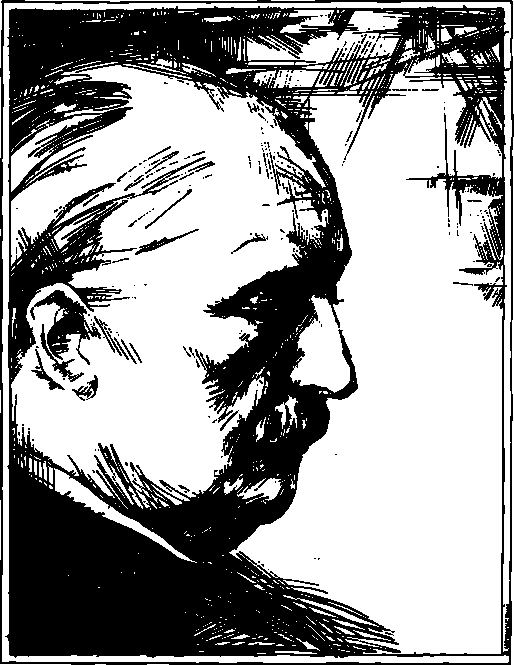
\includegraphics[width=0.8\textwidth]{figures/helmholtz.pdf}
\end{center}
{\small \textsf{{Hermann Helmholtz [1821-1894]}} -- \textsf{\footnotesize a famous German scientist. Helm­holtz worked in the fields of physics, mathematics and physiology with great success. He was the first (1847) to give a mathematical interpretation of the law of conservation of energy emphasizing the universal character of this law. Helmholtz obtained outstanding ing results in thermodynamics; he was the first to apply it to the study of chemical processes. By means of his work on the vortex motion of liquids, Helmholtz laid the foundations of hydro-dynamics and aerodynamics. He carried out a number of valuable investigations in the fields of acoustics and electromagnetism. Helmholtz developed the physical theory of music He applied powerful and original mathematical methods m his physical research.}}


The credit for this belongs to the German physicist Hermann Helmholtz. On July 23, 1847, at a meeting of the Berlin Physical Society, Helmholtz gave a lecture on the principle of conservation of energy. The mechanical basis of the law of conservation of energy was clearly presented for the first time in this talk. The world con­sists of atoms; atoms possess potential and kinetic ener­gies. The sum of the potential and kinetic energies of the particles which a body or system is made of cannot change, if the body or system is not subjected to ex­ternal influences. The law of conservation of energy, as we outlined it several pages above, was first formulated by Helmholtz.

After the work of Helmholtz, it remained for other physicists to merely verify and apply the law of conserva­tion of energy. The success of these investigations led to the fact that by the end of the fifties the law of con­servation of energy was universally recognized as fundamental law of natural science.

Phenomena casting doubt on the law of conservation of energy have already been observed in the 20th century. However, explanations were later found for the apparent discrepancies. The law of conservation of energy has so far always stood the test with credit.

%\begin{figure}[!ht]
%\centering
%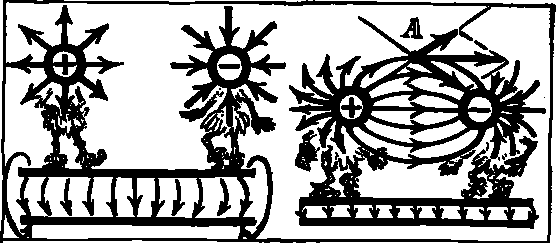
\includegraphics[width=\textwidth]{figures/fig-01-01.pdf}
%\caption{Using springs for measuring weights.}
%\label{fig-1.1}
%\end{figure}



